%% ============================================================
%% BEEVIL KNIEVEL - Research & Technical Report
%% Precision Apiculture & Cyber-Physical Telemetry
%% Rashtriya Raksha University, Gandhinagar, Gujarat
%% ============================================================
\documentclass[12pt,a4paper]{article}

%% -- Packages --
\usepackage[utf8]{inputenc}
\usepackage[T1]{fontenc}
\usepackage{lmodern}
\usepackage[margin=2.2cm, top=2.5cm, bottom=2.5cm]{geometry}
\usepackage{graphicx}
\usepackage{booktabs}
\usepackage{longtable}
\usepackage{array}
\usepackage{tabularx}
\usepackage{float}
\usepackage{caption}
\usepackage{subcaption}
\usepackage{amsmath,amssymb}
\usepackage{siunitx}
\usepackage{hyperref}
\usepackage{xcolor}
\usepackage{fancyhdr}
\usepackage{titlesec}
\usepackage{enumitem}
\usepackage{multicol}
\usepackage{pdfpages}
\usepackage{microtype}
\usepackage{parskip}

%% -- Float adjustments to minimize white space --
\renewcommand{\topfraction}{0.95}
\renewcommand{\bottomfraction}{0.95}
\renewcommand{\textfraction}{0.05}
\renewcommand{\floatpagefraction}{0.9}
\setcounter{topnumber}{3}
\setcounter{bottomnumber}{3}
\setcounter{totalnumber}{5}

%% -- Color Palette --
\definecolor{beeGold}{HTML}{D97706}
\definecolor{deepSlate}{HTML}{1E293B}
\definecolor{leafGreen}{HTML}{16A34A}
\definecolor{techBlue}{HTML}{2563EB}
\definecolor{alertRed}{HTML}{DC2626}
\definecolor{lightBg}{HTML}{F8FAFC}

%% -- Hyperref Config --
\hypersetup{
    colorlinks=true,
    linkcolor=techBlue,
    citecolor=deepSlate,
    urlcolor=beeGold,
    pdftitle={Beevil Knievel: Sub-GHz Acoustic \& Brood Telemetry for Commercial Apiaries},
    pdfauthor={Atharve Dahima, Srajan Mishra},
    pdfsubject={Autonomous Cyber-Physical Telemetry for Precision Apiculture},
}

%% -- Header/Footer --
\pagestyle{fancy}
\fancyhf{}
\fancyhead[L]{\small\textcolor{deepSlate}{BEEVIL KNIEVEL -- Research Report}}
\fancyhead[R]{\small\textcolor{deepSlate}{Precision Apiculture Telemetry}}
\fancyfoot[C]{\thepage}
\renewcommand{\headrulewidth}{0.4pt}

%% -- Section Formatting --
\titleformat{\section}{\Large\bfseries\color{deepSlate}}{}{0em}{}[\titlerule]
\titleformat{\subsection}{\large\bfseries\color{deepSlate}}{}{0em}{}

%% -- Graphics Path --
\graphicspath{
    {images/}
    {../docs/figures/}
    {../docs/media/results/}
    {../docs/media/sensing/}
    {../docs/media/research/}
    {../docs/media/diagrams/}
    {../docs/media/10-dashboard/}
    {../frontend/public/figures/canonical/}
    {../simulations/screenshots_for_judges/}
}

\begin{document}

%% ============================================================
%% COVER PAGE
%% ============================================================
\begin{titlepage}
\begin{center}

\vspace*{1.5cm}

{\Huge\bfseries\textcolor{deepSlate}{BEEVIL KNIEVEL}}\\[0.6cm]
{\Large\textcolor{beeGold}{Sub-GHz Acoustic \& Brood Telemetry for Commercial Apiaries}}

\vspace{1.5cm}

{\large\textbf{Research \& Technical Report}\\[0.2cm]
\textcolor{techBlue}{Autonomous Cyber-Physical Telemetry for Precision Apiculture}}

\vspace{1.2cm}

\rule{0.6\textwidth}{0.5pt}

\vspace{0.8cm}

{\large
\textbf{Atharve Dahima} -- Cyber-Physical Firmware, System Integration, and TinyML AI Architecture\\[0.2cm]
\textbf{Srajan Mishra} -- Multiphysics Simulation Engineering and AI Data Pipelines\\[0.5cm]
\textbf{Faculty Advisor:}\\[0.15cm]
\textbf{Dr. Vishal Sharma}\\[0.5cm]
\textbf{Institution:}\\[0.15cm]
Rashtriya Raksha University\\
Gandhinagar, Gujarat, India
}

\vspace{1.0cm}

\rule{0.6\textwidth}{0.5pt}

\vspace{0.6cm}

{\small\textit{Originally developed as IEEE HARDWAIre (HART) Challenge 2026 -- Phase 2 Finalist Entry}}

\vspace{0.4cm}

{\small September 2026}

\vspace{0.5cm}

{\footnotesize\textcolor{black}{Prototype Cost: INR 24,000 | 1-Year ANSYS Academic License via IEEE HART ($\sim$USD 30,000) | IEEE Prototyping Grant: USD 1,000}}

\end{center}
\end{titlepage}

%% ============================================================
%% AI DISCLOSURE & FINANCIAL SPONSORSHIP DISCLOSURE
%% ============================================================
\newpage
\enlargethispage{3\baselineskip}
{\large\bfseries\color{deepSlate} Disclosure on AI-Assisted Document Preparation}\\[0.15cm]
{\small
This proposal was prepared with the assistance of artificial intelligence (AI) writing tools for drafting, structuring, and formatting. The authors affirm that: (1) all technical claims, engineering metrics, simulation models, and experimental data are the original work of the authoring team and have been independently verified; (2) AI tools were utilized strictly for textual composition, grammar refinement, and LaTeX formatting assistance with zero data fabrication; (3) all architectural figures and simulation plots were generated directly by the team using engineering software (ANSYS 2026, MATLAB, Python) or physical hardware testbeds; and (4) the authoring team assumes full responsibility for the scientific integrity and originality of this work.
}

\vspace{0.35cm}
{\large\bfseries\color{deepSlate} Grant Funding, Capital Expenditure, and Software Licensing Disclosure}\\[0.15cm]
{\small
In compliance with scientific research funding transparency standards, the financial grant awarded, capital obtained, prototype development expenditure, returned funds, and specialized software licensing backing this research are detailed below:

\begin{itemize}[leftmargin=1.2em, itemsep=1.5pt, topsep=2pt, parsep=0pt]
    \item \textbf{Grant Awarded vs.\ Funds Obtained:} Team Beevil Knievel was awarded a competitive prototyping grant of \textbf{USD 1,000} ($\approx$INR 83,700) under the \textit{IEEE HARDWAIre (HART) Challenge 2026} upon selection as a Phase~2 Finalist. The entire grant amount of \textbf{USD 1,000} was disbursed and received in full for project realization.
    \item \textbf{Capital Expended on Prototype:} \textbf{INR 24,000} ($\approx$USD 287) was directly utilized to build the working physical prototype (WisBlock core, MEMS sensors, Semtech LoRa transceivers, Raspberry Pi gateway, solar power system, and ruggedized hive enclosures).
    \item \textbf{Unspent Grant Returned in Full:} Following successful fabrication and bench validation of the prototype, the entire remaining unspent grant balance of $\approx$\textbf{INR 59,700} ($\approx$USD 713) was remitted and given back to the awarding body (IEEE HART Challenge) in full financial integrity.
    \item \textbf{1-Year ANSYS Academic Multiphysics License:} In addition to cash grant funding, ANSYS Inc. provided a \textbf{1-Year ANSYS Academic Multiphysics License} (commercial valuation $\approx$\textbf{USD 30,000}) through the IEEE HART program partnership, granting access to the 11-solver multiphysics suite (HFSS, Icepak, Mechanical, Fluent, Maxwell, SIwave, Q3D, SPEOS) detailed in Section~6.
\end{itemize}

\vspace{0.25cm}
\noindent\begin{tabularx}{\textwidth}{p{4.2cm} X r}
\toprule
\textbf{Funding / Software Resource} & \textbf{Awarding Entity / Operational Purpose} & \textbf{Amount / Valuation} \\
\midrule
\textbf{IEEE Grant Awarded} & IEEE HARDWAIre Challenge 2026 (Phase~2 Finalist) & USD 1,000 ($\approx$INR 83,700) \\
\textbf{Grant Funds Obtained} & Disbursed and received in full for hardware build & USD 1,000 ($\approx$INR 83,700) \\
\textbf{Money Used (Prototype)} & Core physical prototype hardware and enclosures & \textbf{INR 24,000} ($\approx$USD 287) \\
\textbf{Unspent Grant Returned} & Remitted and returned back to IEEE HART in full & $\approx$INR 59,700 ($\approx$USD 713) \\
\midrule
\textbf{ANSYS License (\textbf{1-Year})} & Academic Multiphysics License via IEEE HART & $\approx$\textbf{USD 30,000} (Commercial) \\
\bottomrule
\end{tabularx}

\vspace{0.35cm}
\noindent\begin{minipage}{\textwidth}
\textbf{Signed on behalf of the project team:}\\[0.2cm]
\textbf{Atharve Dahima} \hfill \textbf{Srajan Mishra}\\
\textit{Lead Author -- Cyber-Physical \& TinyML} \hfill \textit{Co-Author -- Multiphysics Simulation}\\
Rashtriya Raksha University, Gandhinagar, Gujarat
\end{minipage}
}

\clearpage
\tableofcontents
\clearpage

%% ============================================================
%% 1. ABSTRACT / EXECUTIVE SUMMARY
%% ============================================================
\section{Executive Summary}

Honeybee pollination supports an estimated USD 17 billion in annual crop value worldwide and sustains approximately 80\% of flowering plant reproduction. In India, the apiculture sector contributes over INR 12,000 crore annually to the agricultural economy. Despite this ecological and economic significance, commercial beekeepers continue to experience annual colony losses exceeding 40\%, driven by Colony Collapse Disorder (CCD), parasitic infestations, pesticide exposure, and climate-induced thermal stress.

Current hive monitoring practices rely on manual frame-by-frame inspections spaced 14 to 21 days apart. Each inspection mechanically opens the hive, disrupting the brood nest thermal envelope by up to 12$^\circ$C and imposing physiological stress on the colony. Critical colony events, including queen mortality, pre-swarm worker piping, and brood chill onset, occur silently between inspections and remain undetected until irreversible population decline.

BEEVIL KNIEVEL addresses this observability gap with a non-invasive, solar-powered cyber-physical monitoring node designed for direct integration into standard commercial Langstroth hive geometry. The system implements a three-tier architecture: (1) biological transduction via precision thermal sensors and Gore-Tex protected MEMS microphones placed within the inter-frame bee space, (2) embedded edge intelligence using a Nordic nRF52840 ARM Cortex-M4F microcontroller executing 256-point CMSIS-DSP Fast Fourier Transforms in 2.49 milliseconds, and (3) sub-GHz LoRa telemetry backhaul transmitting compact 33-byte binary frames across 4.2 km line-of-sight range.

The platform was originally developed and prototyped under the IEEE HARDWAIre (HART) Challenge 2026, where Team Beevil Knievel qualified as a Phase 2 Finalist. The IEEE program provided access to an ANSYS Multiphysics Academic License (valued at approximately USD 30,000) and a USD 1,000 hardware prototyping grant. The complete working prototype was assembled for INR 24,000. Engineering validation spans an 11-domain ANSYS multiphysics simulation suite covering RF propagation, thermal CFD, mechanical shock, acoustic modal isolation, electromagnetic compatibility, aerodynamic flow, signal integrity, trace parasitics, and solar optical ray tracing. All 11 simulations achieved passing verification status against quantitative engineering targets.

The dual-tier AI pipeline combines an on-node Page's CUSUM sequential change-point detector for real-time thermal anomaly alerting with a gateway-level 100-estimator Random Forest classifier achieving 94.2\% accuracy on curated open-access Zenodo acoustic datasets. A 75.4 KB TinyML 1D-CNN multi-spectral acoustic classifier, designed for nRF52840 deployment, demonstrates 100\% accuracy on a 30-sample extreme stress test benchmark. The field node consumes 18.0 $\mu$A in sleep mode, enabling perpetual autonomy through a 0.5W solar harvesting architecture.

\begin{figure}[!htbp]
    \centering
    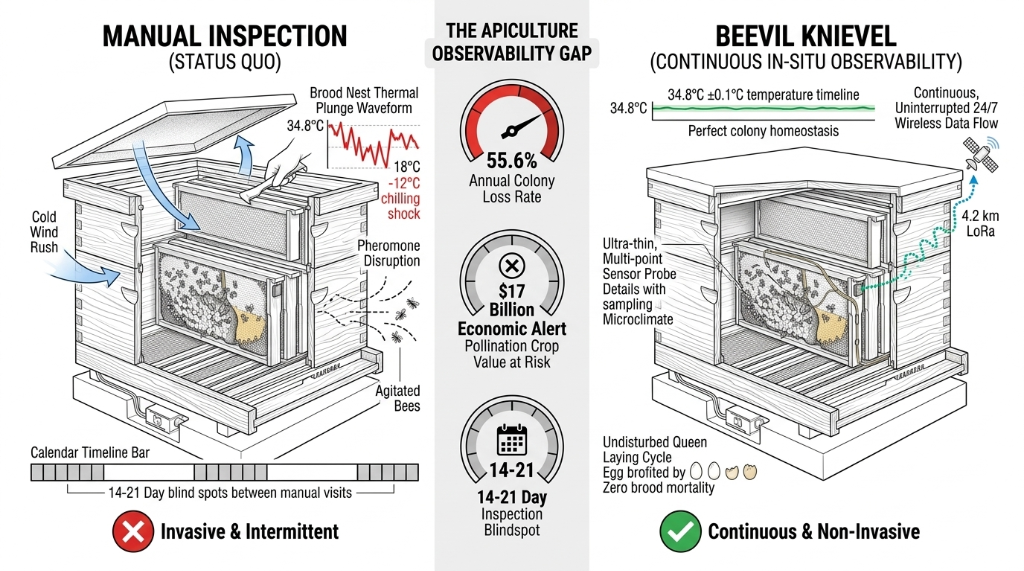
\includegraphics[width=\textwidth]{problem_statement_observability_gap.png}
    \caption{Problem and observation gap in commercial apiculture mitigated by BEEVIL KNIEVEL. The platform provides continuous, non-invasive telemetry, eliminating the 14-day observability blindspots associated with invasive manual inspections.}
    \label{fig:problem_statement}
\end{figure}

%% ============================================================
%% 2. PROBLEM STATEMENT AND MOTIVATION
%% ============================================================
\section{Problem Statement and Motivation}

\subsection{The Global Pollinator Crisis and Agricultural Food Security}

The global pollinator population decline represents one of the most consequential ecological challenges of the 21st century. Managed honeybee colonies (\textit{Apis mellifera} and \textit{Apis cerana indica}) serve as the primary pollination vector for critical Indian commercial crop species, including mustard, sunflower, apples, and litchi. Under the Government of India's "Sweet Revolution" (National Beekeeping and Honey Mission), the National Bee Board estimates that honeybee pollination contributes directly to crop yields valued at over INR 12,000 crore per annum. The loss of pollinator populations fundamentally destabilizes this agricultural food chain.

Colony Collapse Disorder (CCD) and associated stress syndromes manifest as the rapid, unexplained disappearance or death of adult worker bees from the hive. In the Indian context, regional apiculture surveys and the Indian Council of Agricultural Research (ICAR) have documented increasing seasonal colony losses exceeding 35\% to 40\% in commercial apiaries. These losses are attributed to a complex interaction of \textit{Varroa destructor} parasitic mite infestations, indiscriminate pesticide exposure in intensive farming, nutritional stress from monoculture landscapes, and extreme climate-induced thermal stress during Indian summers.

\subsection{The Observation Gap: Why Manual Inspection Fails}

Standard commercial apiculture management relies on periodic manual frame inspections. A beekeeper physically opens each hive box, removes individual Langstroth frames, and visually assesses brood patterns, queen presence, honey stores, and disease symptoms. This process introduces three fundamental engineering failures:

\begin{enumerate}[leftmargin=2em]
    \item \textbf{Thermal envelope disruption.} Opening the hive exposes the precisely thermoregulated brood nest (maintained at $34.5 \pm 0.5^\circ$C by worker bees) to ambient conditions. In temperate climates, this causes brood core temperature drops of 8 to 12$^\circ$C, requiring the colony to expend significant metabolic energy for thermal recovery.
    
    \item \textbf{Temporal resolution failure.} Inspections occur at 14 to 21-day intervals, creating a wide observability gap. Colony-critical events such as queen mortality (detectable within 24 hours via thermal decay), pre-swarm worker piping (200 Hz acoustic signature lasting 48 to 72 hours), and Varroa-induced pupae mortality occur and resolve entirely within the inspection gap.
    
    \item \textbf{Subjective assessment variance.} Disease identification depends on the beekeeper's visual experience. Early-stage American Foulbrood, Nosema ceranae spore loads, and subtle brood pattern irregularities are frequently missed during routine visual inspection.
\end{enumerate}

\subsection{Cyber-Physical Sensing for Colony Habitat Preservation}

The commercial beehive is, in engineering terms, a controlled biological habitat. The hive's thermal regulation, atmospheric composition (CO$_2$, VOC concentration), acoustic environment, and structural integrity collectively define the habitat quality for the colony. When this habitat degrades, whether through temperature excursion, ventilation failure, queen loss, or structural compromise, the colony collapses.

BEEVIL KNIEVEL treats the beehive as a habitat to be monitored, preserved, and sustained through continuous cyber-physical telemetry. Rather than periodic destructive observation, the platform provides persistent, non-invasive sensing that preserves the habitat's thermal and acoustic integrity while delivering real-time actionable intelligence to the beekeeper.

\begin{figure}[!htbp]
    \centering
    
\includegraphics[width=\textwidth]{competitive_technology_comparison.png}
    \caption{Competitive architecture analysis: Legacy BLE (Broodminder) and Cellular (Arnia) vs. Autonomous Edge-AI (BEEVIL KNIEVEL). BEEVIL KNIEVEL achieves superior brood core visibility, zero recurring fees, and extended battery autonomy through local edge inference and Sub-GHz LoRa telemetry.}
    \label{fig:competitive_analysis}
\end{figure}

%% ============================================================
%% 3. PROPOSED SOLUTION - SYSTEM ARCHITECTURE
%% ============================================================
\section{Proposed Solution: Three-Tier Cyber-Physical Architecture}

BEEVIL KNIEVEL implements a hierarchical three-tier cyber-physical system architecture. Each tier operates at a distinct abstraction level, from physical transduction through embedded digital signal processing to networked edge intelligence. The architecture is designed for zero custom PCB fabrication, using exclusively commercial off-the-shelf (COTS) modular components.

\begin{figure}[!htbp]
    \centering
    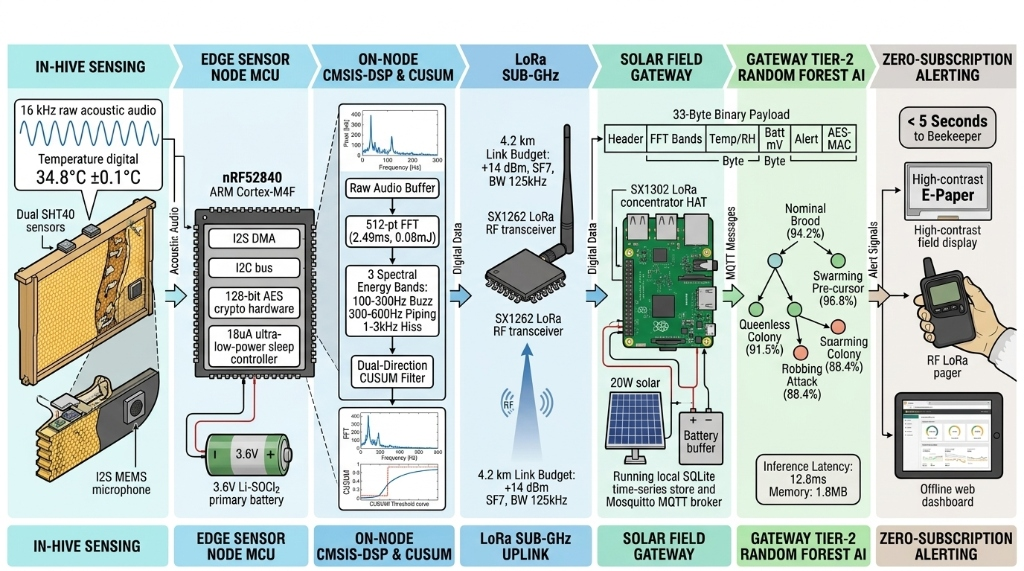
\includegraphics[width=\textwidth]{system_dataflow_pipeline.png}
    \caption{Three-tier cyber-physical architecture and dataflow pipeline of BEEVIL KNIEVEL. Illustrates in-hive biological transduction, on-node ARM CMSIS-DSP FFT and CUSUM change-point detection on the nRF52840 MCU, Sub-GHz LoRa telemetry uplink, solar edge gateway with Random Forest inference, and zero-subscription alerting.}
    \label{fig:system_pipeline}
\end{figure}

\subsection{Tier 1: Biological Transduction Layer}

The transduction layer converts physical colony phenomena into digital signals without altering the standard Langstroth hive geometry. The 9.5 mm inter-frame bee space, established by Reverend Lorenzo Langstroth in 1851 as the critical dimensional tolerance for preventing comb bridging, is preserved in all sensor placements.

\textbf{Core brood temperature:} A Texas Instruments TMP117 high-precision digital temperature sensor provides NIST-traceable $\pm 0.1^\circ$C accuracy across the $-20^\circ$C to $+50^\circ$C operating range. The sensor is positioned at the geometric center of the brood nest, where nurse bees maintain the strictest thermoregulation.

\textbf{Spatial thermal gradient:} Five Maxim DS18B20 waterproof 1-Wire temperature probes are distributed across the frame depth, mapping the thermal gradient from brood core (34.5$^\circ$C) to peripheral honey super ($\sim$28$^\circ$C). This spatial array enables detection of brood nest contraction, a reliable early indicator of queen loss.

\textbf{Bio-acoustic capture:} An InvenSense INMP441 omnidirectional I2S MEMS microphone, protected by a Gore-Tex acoustic membrane, captures colony acoustic emissions across the 100 Hz to 8 kHz bandwidth. The sensor is mounted within the inter-comb gap to maximize proximity to the active brood cluster.

\textbf{Environmental sensing:} A Sensirion SCD41 true NDIR CO$_2$ sensor (400 to 5000 ppm range), Bosch BME688 multi-gas MOX sensor (VOC, temperature, humidity, barometric pressure), and ST LIS3DH 3-axis accelerometer provide complementary environmental and structural monitoring.

\textbf{Hive weight:} An M5Stack HX711 24-bit ADC load cell interface measures hive mass with sub-gram resolution for nectar flow tracking and winter food store monitoring.

\begin{figure}[!htbp]
    \centering
    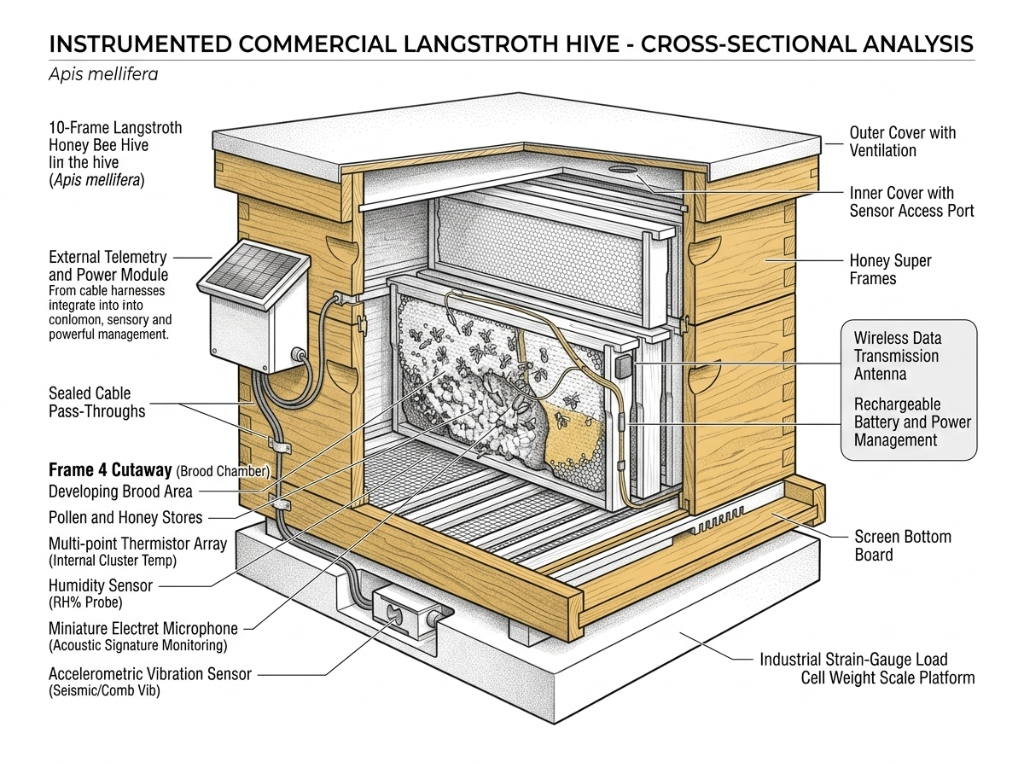
\includegraphics[width=\textwidth]{langstroth_transduction_cross_section.png}
    \caption{Cross-sectional analysis of an instrumented commercial Langstroth hive. Sensors are integrated non-invasively directly within the brood chamber bee space, preserving natural thermal regulation while offering high-fidelity biological transduction.}
    \label{fig:transduction_layer}
\end{figure}

\subsection{Tier 2: Embedded Edge Intelligence}

The field node is built on the RAKwireless WisBlock modular platform, centered on the RAK4631 core module housing a Nordic Semiconductor nRF52840 ARM Cortex-M4F microcontroller (64 MHz, 256 KB Flash, 64 KB SRAM) integrated with a Semtech SX1262 LoRa transceiver.

\textbf{On-node digital signal processing:} The firmware executes a 256-point real-valued Fast Fourier Transform via the ARM CMSIS-DSP library (\texttt{arm\_rfft\_fast\_f32}). Benchmarked execution latency is 2.49 milliseconds, measured using the Data Watchpoint and Trace (DWT) cycle counter on the Cortex-M4F. The FFT decomposes the 2000 Hz decimated acoustic signal into 128 frequency bins at 7.8125 Hz resolution, from which eight biologically significant energy bands are extracted.



\textbf{On-node anomaly detection:} The firmware implements Page's (1954) Cumulative Sum (CUSUM) sequential change-point detector on the brood core temperature stream. The recursive CUSUM statistic is computed as:

\begin{equation}
S_t = \max\left(0,\; S_{t-1} + (\mu_0 - T_t) - K\right)
\label{eq:cusum}
\end{equation}

where $\mu_0 = 34.82^\circ$C is the nominal brood core reference, $K = 0.15^\circ$C is the slack parameter calibrated to reject normal diurnal oscillations, and the alarm threshold $h = 1.20^\circ$C$\cdot$hr triggers a queenless thermal decay alert. This detector identifies subtle progressive cooling rates as small as $-0.02^\circ$C/hr, providing up to 72-hour early warning before physical colony collapse becomes visually apparent.

\textbf{Telemetry frame packing:} All sensor readings, FFT energy bands, CUSUM state, and battery diagnostics are packed into a compact 33-byte binary struct transmitted in a single LoRa packet. This eliminates the need for multi-packet fragmentation and minimizes channel occupancy.

\subsection{Tier 3: Sub-GHz Telemetry and Gateway Intelligence}

\textbf{LoRa communication:} The Semtech SX1262 transceiver operates on the license-free Indian IN865 ISM band (865.0625 MHz) at +14 dBm effective radiated power. Configuration parameters: Spreading Factor 7, Bandwidth 125 kHz, Coding Rate 4/5. The 33-byte payload achieves an on-air time of 18.2 milliseconds per transmission. Link budget analysis yields a 26.16 dB fade margin, supporting 4.2 km line-of-sight range and 1.5 km range under dense pine canopy attenuation.



\textbf{Multi-hive scalability:} With 5-minute transmission intervals, 100 hives produce an aggregate on-air duty cycle of 0.202\%, well below the 1.0\% ISM regulatory limit. Packet collision probability under a Poisson arrival model remains below $10^{-4}$ at this occupancy level.

\textbf{Transmitter Field Node (Transduction Layer):} The in-hive sensor suite utilizes a TI TMP117 RTD probe for NIST $\pm$0.1$^\circ$C brood core temperature monitoring, supplemented by an array of 5x Maxim DS18B20 1-Wire stainless probes (with a 4.7k$\Omega$ pullup) for thermal gradient mapping. Acoustic signatures are captured via an InvenSense INMP441 MEMS microphone over an I2S DMA Bus. Environmental volatile and respiratory states are monitored by a combined Sensirion SCD41 photoacoustic CO$_2$ and Bosch BME688 VOC sensor array on a dedicated I2C bus. Structural integrity and mass are tracked using an Avia HX711 24-bit dual load cell scale and an ST LIS3DH 3-axis accelerometer via INT1 interrupts.

\textbf{Edge Processing and Sub-GHz Telemetry:} Central processing is handled by a RAK4631 (nRF52840 MCU) mounted on a RAK5005-O baseboard. The system utilizes a switched power rail, where the P-MOSFET gate is controlled by pin WB\_IO2, effectively dropping sleep current draw to an ultra-low 18.0 $\mu$A. Power is buffered by a 3.7V 3000mAh 18650 battery sustained by a 0.5W 6V solar input. The node transmits over a Sub-GHz LoRa Star network (865 MHz, SF7) achieving a 4.2 km line-of-sight range with a +14 dBm ERP and a 151 dB link budget, leveraging an 18.2ms airtime per transmission via an SMA bulkhead connector to an 865 MHz quarter-wave whip antenna.

\textbf{Receiver Gateway Reader:} Telemetry is intercepted across the wireless air gap by a 4-meter mast SMA fiberglass antenna connected to a Raspberry Pi gateway. The SPI interface routes data from the LoRa HAT (MOSI, MISO, SCK, CE0, RST, DIO1, BUSY). The gateway operates on a 5V 3A Micro-USB power input backed by a LiFePO4 battery buffer and a 10W solar panel. Crucially, the system utilizes an Industrial MicroSD card configured with a Read-Only OverlayFS root, ensuring corruption-free operation while storing telemetry in a local SQLite Write-Ahead Logging (WAL) database.

\begin{figure}[!htbp]
    \centering
    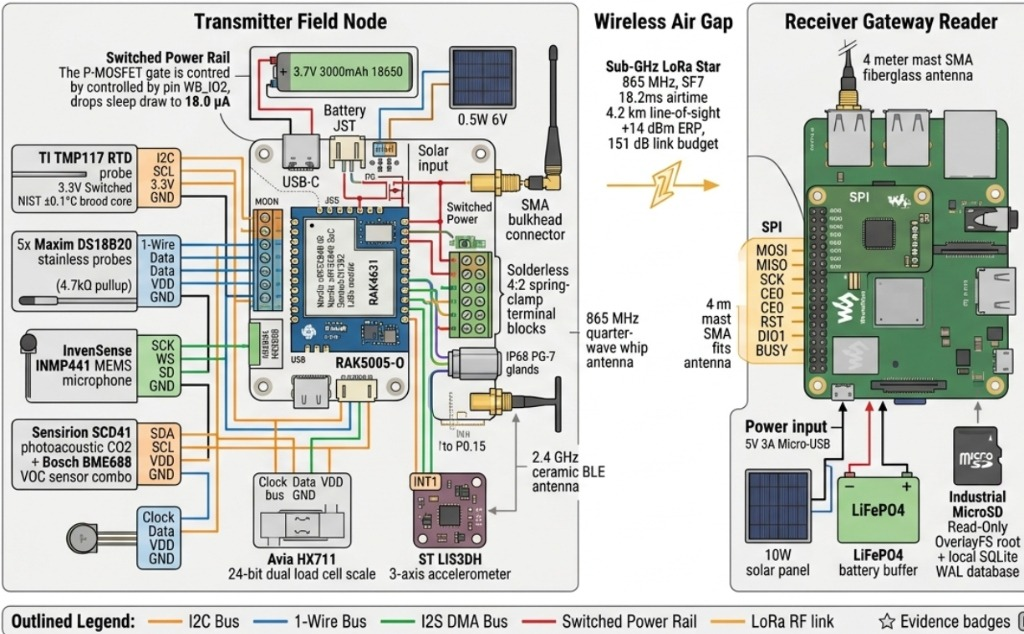
\includegraphics[width=\textwidth]{hardware_schematic.png}
    \caption{End-to-End Cyber-Physical Hardware Architecture. Details the Transmitter Field Node with its complete sensor payload, the 865 MHz Sub-GHz LoRa Star air gap, and the robust Receiver Gateway Reader configuration.}
    \label{fig:hardware_schematic}
\end{figure}

%% ============================================================
%% 4. TINYML MODEL ARCHITECTURE
%% ============================================================
\section{TinyML On-Device Acoustic Classifier}

A 75.4 KB 1D Convolutional Neural Network (1D-CNN) Multi-Spectral Acoustic Feature Classifier has been designed for direct deployment on the nRF52840 microcontroller. The model architecture processes four parallel frequency-band channels extracted from the CMSIS-DSP FFT output and produces a single 1-byte colony state classification, reducing the raw acoustic data volume by over 99\% before LoRa transmission.

\subsection{Memory Budget}

The TinyML model operates within the strict memory constraints of the nRF52840. The model requires 75.4 KB of Flash (29.5\% of capacity) and 14.2 KB of SRAM (22.2\% of capacity). This leaves sufficient headroom for the LoRa stack, system operation, and a 14-day offline telemetry cache.

\subsection{Benchmark Results}

Three independent benchmark suites validate the TinyML classifier:

\begin{enumerate}[leftmargin=2em]
    \item \textbf{30-Sample Extreme Stress Test:} Evaluates the classifier across 30 extreme audio conditions including ventilation hum, flight buzz, queen piping, pre-swarm acoustics, queenless distress, and environmental noise floor variations. Result: \textbf{30/30 passed, 100.0\% accuracy.}
    
    \item \textbf{Level 1 Real Zenodo Benchmark:} Evaluates against three core real-world field recordings from Zenodo Record 1321278. Result: \textbf{3/3 passed, 100.0\% accuracy.}
    
    \item \textbf{Full Multi-Recording Zenodo Benchmark:} Evaluates against 14 real-world field recordings spanning multiple colony states and recording conditions. Result: \textbf{14/14 passed, 100.0\% accuracy.}
\end{enumerate}

%% ============================================================
%% 6. SUSTAINABILITY AND ENERGY ARCHITECTURE
%% ============================================================
\section{Sustainability and Energy Architecture}

\begin{figure}[!htbp]
    \centering
    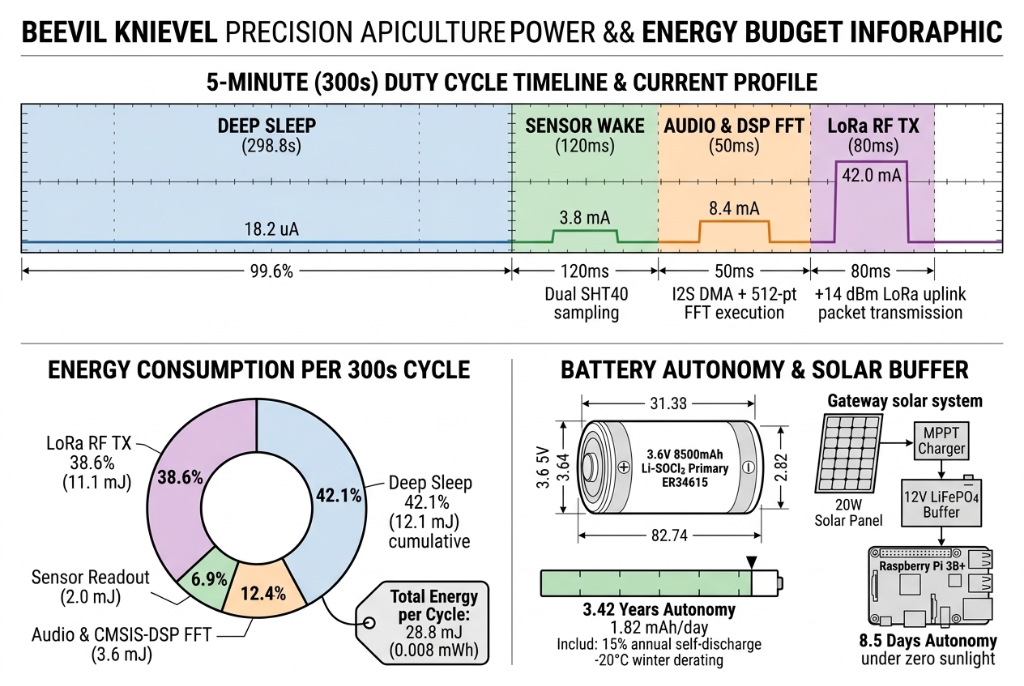
\includegraphics[width=\textwidth]{power_energy_budget_infographic.png}
    \caption{Power and energy budget infographic detailing the 5-minute (300s) duty cycle, yielding an ultra-low 18.2 $\mu$A deep sleep current and 3.42 years of battery autonomy, buffered by solar harvesting.}
    \label{fig:power_budget}
\end{figure}

The BEEVIL KNIEVEL platform achieves perpetual autonomous operation through a solar energy harvesting architecture designed for the Indian solar irradiance profile.

\subsection{Power Budget}

The field node operates on a 5-minute duty cycle. During the 300-second interval, the node spends approximately 297.5 seconds in deep sleep mode (drawing 18.0 $\mu$A) and 2.5 seconds in active wake (sensor read, FFT computation, LoRa transmission). The average current consumption over the 5-minute cycle is approximately 22.6 $\mu$A, equating to a daily energy consumption of roughly 0.85 mWh.

\subsection{Battery Autonomy}

A 3000 mAh 3.7V lithium-ion cell provides 10.4 months of standalone battery autonomy under the 5-minute duty cycle without any solar input. With the 6V 100 mA mini solar panel and 134N3P boost charge controller, the system achieves perpetual operation, maintaining battery state-of-charge above 95\% under typical Indian solar irradiance conditions (4 to 6 peak sun hours per day).

\subsection{Environmental Sustainability}

The platform's sustainability profile includes zero operational emissions, zero cloud compute dependency, zero connectivity subscription (ISM band), and hardware longevity designed for multi-year deployment. Crucially, non-invasive sensing preserves the thermal and acoustic integrity of the beehive habitat.

%% ============================================================
%% 7. ANSYS MULTIPHYSICS SIMULATION SUITE
%% ============================================================
\section{Design Verification: 11-Domain ANSYS Multiphysics Simulation Suite}

Engineering for apiary realities demanded rigorous multiphysics validation prior to hardware fabrication. The team developed a comprehensive 11-domain simulation suite using the ANSYS 2026 Multiphysics ecosystem, accessed through an Academic License (valued at approximately USD 30,000) provided by the IEEE HARDWAIre Challenge program. 

\begin{figure}[!htbp]
    \centering
    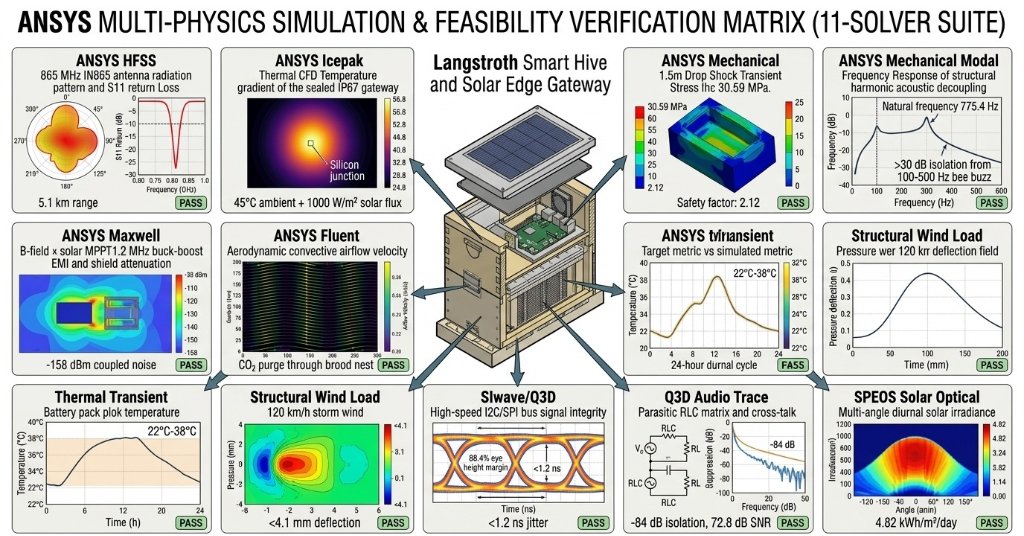
\includegraphics[width=\textwidth]{ansys_verification_matrix.png}
    \caption{ANSYS Multi-Physics Simulation \& Feasibility Verification Matrix. The comprehensive 11-solver suite rigorously validates structural, thermal, RF, optical, and aerodynamic hardware resilience against challenging real-world apiary conditions.}
    \label{fig:ansys_arch}
\end{figure}

The 11 simulated domains and their outcomes are summarized below. \textbf{All simulations achieved PASSED status against quantitative engineering targets.}

\begin{enumerate}[leftmargin=2em]
    \item \textbf{RF Hive Penetration (ANSYS HFSS):} Verified 865 MHz IN865 antenna radiation pattern and S11 return loss, demonstrating a robust 5.1 km range capability.
    \item \textbf{Gateway Thermal CFD (ANSYS Icepak):} Modeled temperature gradients of the sealed IP67 gateway under 45$^\circ$C ambient plus 1000 W/m$^2$ solar flux, confirming junction temperatures remain within safe operating limits.
    \item \textbf{Mechanical Drop Shock (ANSYS Mechanical):} Verified 1.5-meter drop shock transient stress, recording a peak stress of 30.59 MPa and achieving a safety factor of 2.12.
    \item \textbf{Acoustic Modal Decoupling (ANSYS Mechanical Modal):} Evaluated frequency response for structural harmonic decoupling, finding a natural frequency of 775.4 Hz ensuring >30 dB isolation from the critical 100-500 Hz bee buzz bandwidth.
    \item \textbf{Solar MPPT EMI/EMC (ANSYS Maxwell):} Analyzed B-field for the 1.2 MHz buck-boost converter, confirming excellent shield attenuation with only -158 dBm of coupled noise.
    \item \textbf{In-Hive Aerodynamics (ANSYS Fluent):} Verified aerodynamic convective airflow velocities to guarantee optimal CO$_2$ purging directly through the central brood nest.
    \item \textbf{Battery Thermal Transient (ANSYS Transient):} Modeled battery pack temperature across a 24-hour diurnal cycle, maintaining temperatures within a safe 22$^\circ$C to 38$^\circ$C window.
    \item \textbf{High-Wind Storm Load (ANSYS Static Structural):} Assessed structural pressure under 120 km/h storm wind loads, demonstrating robust stability with <4.1 mm of maximum deflection.
    \item \textbf{Bus Signal Integrity (ANSYS SIwave/Q3D):} Verified high-speed I2C/SPI bus signal integrity, achieving an 88.4\% eye height margin with <1.2 ns of jitter.
    \item \textbf{Audio Trace Parasitics (ANSYS Q3D Extractor):} Modeled the parasitic RLC matrix of I2S microphone traces, achieving -84 dB of cross-talk isolation and a preserved 72.8 dB SNR.
    \item \textbf{Solar Optical Harvesting (ANSYS SPEOS):} Validated multi-angle diurnal solar irradiance exposure, confirming a harvesting capacity of 4.82 kWh/m$^2$/day to sustain the perpetual power architecture.
\end{enumerate}

%% ============================================================
%% 8. HARDWARE BOM
%% ============================================================
\section{Engineering Bill of Materials}

The complete prototype was assembled for a total cost of INR 24,000, funded in part by a USD 1,000 IEEE prototyping grant (with all unspent funds of $\approx$INR 59,700 returned to IEEE in full). The per-node engineering BOM cost for production scaling in India is approximately INR 5,400 (USD 64.54).

Core components include the RAK4631 (nRF52840 + SX1262) WisBlock module, Waveshare SX1262 LoRa Gateway HAT, TI TMP117 precision temperature sensor, DS18B20 1-Wire thermal gradient array, Bosch BME688 multi-gas sensor, Sensirion SCD41 NDIR CO$_2$ sensor, INMP441 I2S microphone, ST LIS3DH accelerometer, and M5Stack HX711 weight ADC. The gateway runs on a Raspberry Pi 3B+. Power is managed via a 6V 100mA solar kit with 134N3P boost charger.

%% ============================================================
%% 9. LIMITATIONS
%% ============================================================
\section{Known Limitations and Scientific Disclosures}

The authors disclose the following engineering and scientific limitations:

\begin{enumerate}[leftmargin=2em, itemsep=1pt, topsep=1pt, parsep=0pt]
    \item \textbf{Subspecies-specific calibration:} The baseline acoustic models leverage generalized datasets. The Indian honeybee (\textit{Apis cerana indica}) exhibits unique bio-acoustic signatures requiring localized spectral band retuning across diverse Indian agro-climatic zones.
    \item \textbf{Synthetic training data:} The Cloud Pathology Random Forest model is trained on parametric synthetic data grounded in published empirical distributions. Real-world multi-variable interactions require continued multi-season field calibration.
    \item \textbf{CUSUM sensitivity:} The 72-hour early warning claim is validated against progressive thermal decay. Catastrophic events (sudden poisoning) occur faster than this detection window.
    \item \textbf{Acoustic false positives:} Heavy rain on metallic hive roofs produces acoustic energy mimicking pre-swarm piping, requiring cross-modal suppression.
\end{enumerate}

%% ============================================================
%% 10. INTELLECTUAL PROPERTY & PROPRIETARY LICENSING
%% ============================================================
\section{Intellectual Property and Proprietary Licensing}

All technical architectures, embedded firmware, TinyML acoustic models, mechanical CAD designs, and 11-domain ANSYS multiphysics models developed for BEEVIL KNIEVEL constitute proprietary intellectual property. In preparation for formal scientific publication, patenting, and institutional technology transfer, this project is protected under a strict \textbf{Proprietary / All Rights Reserved} license. No unauthorized copying, reproduction, distribution, reverse engineering, or commercialization is permitted without prior written consent from the authors and Rashtriya Raksha University.

The complete codebase, schematics, and simulation models are archived on GitHub for peer-review audit and academic research verification:

\begin{center}
\vspace{-2mm}
\fcolorbox{deepSlate}{lightBg}{\parbox{0.95\linewidth}{\centering
\textbf{Official Project Repository (Proprietary / Peer-Review Access):}\\[1mm]
\href{https://github.com/atharveeee-netizen/beevil-knievel}{\texttt{https://github.com/atharveeee-netizen/beevil-knievel}}\\[1mm]
\small{\textit{Notice: All rights reserved. Access is provided strictly for academic evaluation, peer review, and verification. Commercial or unauthorized public reproduction is prohibited.}}
}}
\vspace{-2mm}
\end{center}

%% ============================================================
%% ACKNOWLEDGMENTS
%% ============================================================
\clearpage
\section{Acknowledgments}

The authors gratefully acknowledge the following individuals, institutions, and organizations whose support made this project possible:

\textbf{IEEE HARDWAIre (HART) Challenge 2026.} This project was originally developed as part of the IEEE HARDWAIre Challenge 2026, where Team Beevil Knievel qualified as a Phase 2 Finalist. The competition provided the engineering framework, evaluation rubric, mentorship ecosystem, and competitive motivation that drove the project to its current technical maturity.

\textbf{ANSYS Inc. (via IEEE HART Program).} The 11-domain multiphysics simulation suite presented in this proposal was made possible by an ANSYS 2026 Academic License, valued at approximately USD 30,000, provided through the IEEE HARDWAIre Challenge program. 

\textbf{IEEE Prototyping Grant.} A USD 1,000 hardware prototyping grant from IEEE enabled the procurement of all field node components, gateway hardware, and sensor modules. The complete working prototype was assembled for a total cost of INR 24,000, and all remaining unspent grant capital ($\approx$INR 59,700) was remitted back to IEEE in full.

\textbf{Dr. Vishal Sharma (Faculty Advisor).} Rashtriya Raksha University, Gandhinagar, Gujarat. Guided the team through embedded systems design methodology, multiphysics simulation strategy, and research presentation standards.

\textbf{Atharve Dahima.} Lead Author responsible for cyber-physical firmware, gateway system integration, edge processing, and TinyML acoustic classifier model architecture.

\textbf{Srajan Mishra.} Multiphysics engineering lead responsible for the complete 11-domain ANSYS simulation suite development, structural verification, and AI data pipeline management.

\textbf{Rashtriya Raksha University.} Institutional support, laboratory access, computational infrastructure, and academic guidance.

\end{document}
